\chapter{Verigraph}\label{ch:verigraph}

Verigraph~\cite{verigraph} is a new tool for simulating and verifying graph grammars, implemented in the purely functional programming language Haskell\footnote{The source code is available at \url{https://github.com/Verites/verigraph}}. The tool is being developed by the Verites group\footnote{\url{http://www.ufrgs.br/verites}} with two particular objectives. 

  The first one is to have a software tool that serves as an implementation of standard constructions and analysis for graph grammars, which is also as close to the theory as possible. The second, to provide a framework for exploring new ideas and techniques in graph grammars and other category theory related topics~\cite{BezerraETMF2016,Costa2016,CostaETMF2016, Becker2014}.

Regarding category theory, verigraph implements important basic constructions such as coequalizers, coproducts, colimits, pushout complements, initial pushouts, pullbacks, negative application conditions, constraints, among others. The implementation of this constructions follows a very similar approach to the one used in~\cite{Rydeheard1988}, where categorial concepts are implemented as types in ML and constructive proofs of theorems in category theory are built as ML programs.

The implemented categorial constructions are used as basis to implement several graph grammar analyses, such as critical pair analysis~\cite{Lambers2006}, state space generation and model checking~\cite{Becker2014}, concurrent rules generation~\cite{BezerraETMF2016} and higher-order graph transformations~\cite{Machado2015}. They were also used to implement the calculation of occurrence graph grammars, which will be explained in depth on
chapter~\ref{ch:process} and used for test case generation on chapter~\ref{ch:tests}.

The analysis algorithms are implemented in a generic functional style, having the advantage of being very close to the formal definitions, thus making it easier to reason about them and to inspect for correctness. In addition, verigraph benefits from a layered architecture (see Figure~\ref{fig:verigraph:layers}) where it is easy to reuse the same algorithms for other categories different than \cat{TGraph_T}, as long as they implement the contracts given by the type
classes (interfaces) defined on the system. 

Some examples of such type classes are shown on
Figures~\ref{fig:verigraph:morphism-type-class} and \ref{fig:verigraph:cocomplete-type-class}.

\begin{figure}[!ht]
  \centering
  \begin{subfigure}[t]{.5\textwidth}
    \centerline{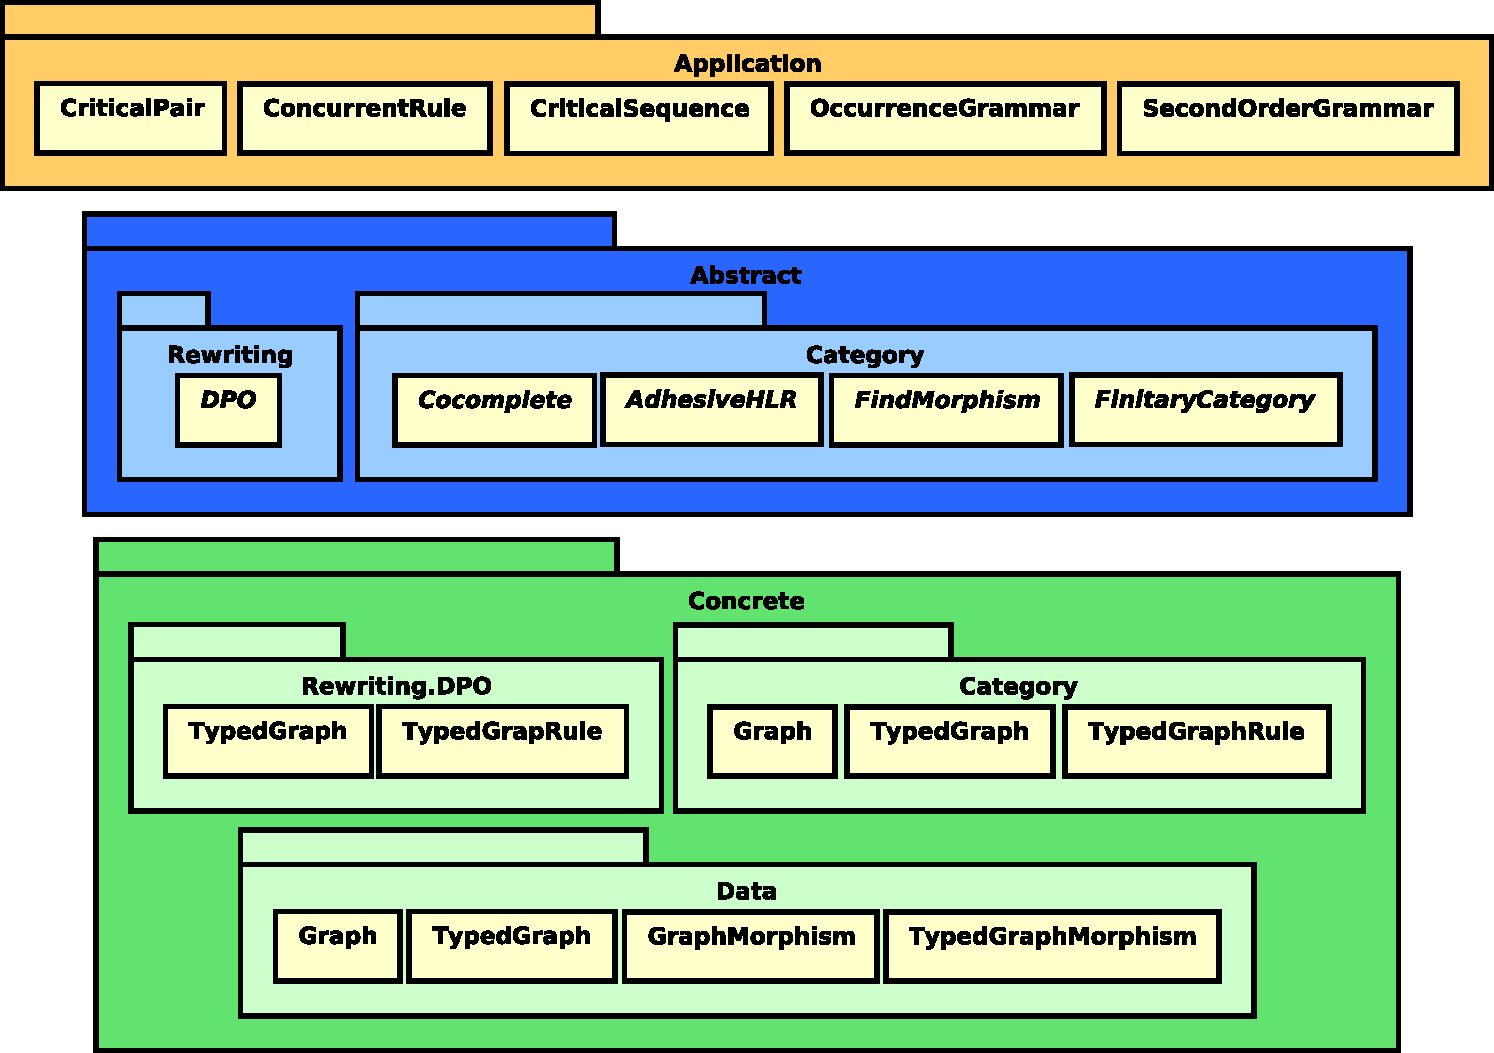
\includegraphics[scale=0.5]{images/verigraph/layers}}
%    \caption{Detailed Layers}
  \end{subfigure}
%  \begin{subfigure}[t]{.5\textwidth}
%    \centerline{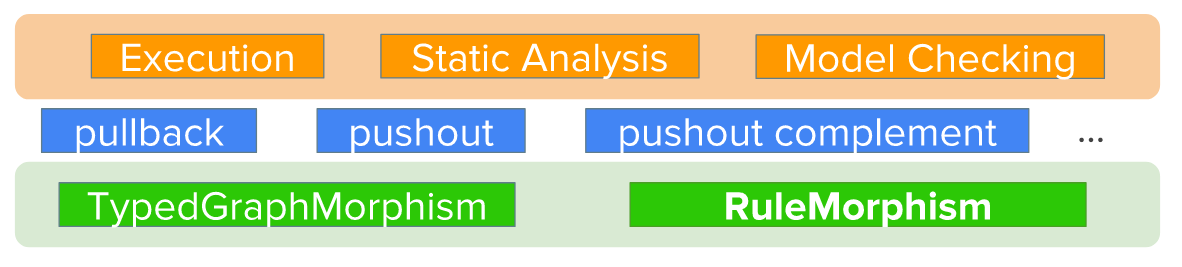
\includegraphics[scale=0.5]{images/verigraph/layers-abstract}}
%    \caption{Example}
%  \end{subfigure}%
  \caption{Verigraph architecture}\label{fig:verigraph:layers}
\end{figure}
There exist tools for analysing graph grammars which are similar to verigraph in some aspects, such as AGG~\cite{Taentzer2000} and GROOVE~\cite{Rensink2004}. However, to our knowledge, Verigraph is the only tool that integrates static and dynamic analyses, second-order specifications and provides support for new categorial constructions and algorithms, besides being the only tool in this field implemented in a pure functional language~\cite{Costa2016}.

Moreover, verigraph is a free and open source software, available online for the community in one of the biggest platform for software repositories currently available. In addition to it, not only its source code, but also its roadmap are public and open to suggestions and collaborations from outside the Verites group.

\section{Implementation of Categorial Constructions}

The first basic type class in Verigraph is \code{Morphism}, shown in Figure~\ref{fig:verigraph:morphism-type-class}, which serves as the minimal contract for any category to be implemented in the tool. Notice how the contract of this type class reflects the category definition (see Definition~\ref{def:category}).

\begin{figure}[!ht]
\caption{Morphism Type Class}
\begin{minted}[linenos=true, breaklines,fontsize=\small]{haskell}
class (Eq m) => Morphism m where
    type Obj m :: *
    compose  :: m -> m -> m
    domain   :: m -> Obj m
    codomain :: m -> Obj m
    id       :: Obj m -> m
    isMonomorphism :: m -> Bool
    isEpimorphism :: m -> Bool
    isIsomorphism :: m -> Bool
\end{minted}
\label{fig:verigraph:morphism-type-class}
\end{figure}

All the other type classes in the tool that are related to category theory are somehow defined in terms of \code{Morphism}. For example, the \code{Cocomplete} type class shown in Figure~\ref{fig:verigraph:cocomplete-type-class} defines some of the most basic categorial constructions used in verigraph, such as coequalizers, coproducts and pushouts.

Notice that, in the \code{Cocomplete} definition, any category that implements the functions \code{calculateCoequalizer} and \code{calculateCoproduct} automatically will have a standard implementation of the \code{calculatePushout} function based only on this two constructions. This is due to the fact that, whenever a category has coequalizers and coproducts, it is possible to calculate any (finite) colimit based only on this two constructions, as demonstrated in~\cite{Pierce1991}.

We took advantage of this result to implement not only the \code{calculatePushout}, but also the calculation of the \code{colimit} of a diagram. The later being used in the calculation of occurrence graph grammars as demonstrated in chapters~\ref{ch:process} and~\ref{ch:tests}.

Another interesting characteristic of the \code{Morphism} type class is that, even though \code{pushouts} and \code{colimits} are implemented in terms of \code{coproducts} and \code{coequalizers}, the programmer can override the default implementation and provide her/his own (categorial specific) implementation. For example, this could be useful when for a given category \cat{C}, a particular algorithm to calculate the pushout is known to more optimized than using the composition of the basic operations.

\begin{figure}[!ht]
  \begin{minted}[linenos=true, breaklines, fontsize=\small]{haskell}
class (Morphism m) => Cocomplete m where

-- | Given two morphisms @/f : A -> B/@ and @/g : A -> B/@ returns the coequalizer morphism
-- @/h : B -> X/@
calculateCoequalizer :: m -> m -> m

-- | Given a non-empty list of morphisms of the form @/f : A -> B/@ returns the coequalizer Morphism
-- @/h : B -> X/@
calculateNCoequalizer :: NonEmpty m -> m

-- | Given two objects @A@ and @B@ it returns the coproduct @(A+B, f: A -> A+B, g: B -> A+B)@
calculateCoproduct :: Obj m -> Obj m -> (m,m)

-- | Given a non-empty list of objects @Bi@ it returns the coproduct @fi : Bi -> SUM(Bi)@
calculateNCoproduct :: NonEmpty (Obj m) -> [m]

calculatePushout :: m -> m -> (m, m)
calculatePushout f g = (f', g')
  where
    b = codomain f
    c = codomain g
    (b',c') = calculateCoproduct b c
    gc' = compose g c'
    fb' = compose f b'
    h = calculateCoequalizer fb' gc'
    g' = compose b' h
    f' = compose c' h
\end{minted}
\caption{Cocomplete Type Class}\label{fig:verigraph:cocomplete-type-class}
\end{figure}

In addition to \code{Morphism}, verigraph has several other important type classes, some examples are:
\begin{itemize}
  \item \code{FindMorphism} for finding morphisms between objects of a category;
  \item \code{AdhesiveHLR} for operations that AdhesiveHLR categories (e.g. \cat{TGraph_T}) are guaranteed to have, such as calculating initial pushouts and pushout complements (when they exist);
  \item \code{DPO} for operations related to DPO graph rewriting approach, such as inversion of rules.
\end{itemize}

Currently, there are three categories implemented on Verigraph: 

\begin{itemize}
  \item \cat{Graph}: graphs as objects and graph morphisms as arrows; 
  \item \cat{TGraph_T}: $T-$typed graphs as objects and $T-$typed graph morphisms as arrows; 
  \item \cat{TSpan_T}: $T-$typed graph morphism spans as objects and span morphisms as arrows (e.g. DPO graph rules and morphisms between rules, respectively).
\end{itemize}

\section{Implementation of Graph Grammars}

The main concrete structures in verigraph are (typed) graph grammars, which is currently the focus of the Verites group. The basic implementation begins with the \code{Graph} type, which consists of a list of nodes and a list of edges together with an API for graph manipulation with basic functions.

The \code{Graph} definition on Haskell is show on Figure~\ref{fig:verigraph:graph}. The API is not shown, but it includes basic graph operations such as \code{insertNode}, \code{insertEdge}, \code{removeNode}, \code{removeEdge}, \code{incomingEdges}, \code{outgoinEdges}, \code{sourceOf}, \code{targetOf}, among others. 

\begin{figure}[!ht]

\caption{Graph implementation}
\begin{minted}[linenos=true, breaklines,fontsize=\small]{haskell}
data Node a = Node 
{ getNodePayload :: Maybe a
} deriving (Show, Read)

data Edge a = Edge 
{ getSource      :: NodeId
, getTarget      :: NodeId
, getEdgePayload :: Maybe a
} deriving (Show, Read)

data Graph a b = Graph 
{ nodeMap :: [(NodeId, Node a)]
, edgeMap :: [(EdgeId, Edge b)]
} deriving (Show, Read)
\end{minted}
\label{fig:verigraph:graph}
\end{figure}

We use \code{Graph} to build the morphisms necessary to implement the categories \cat{Graph}, \cat{TGraph_T} and \cat{TSpan_T}. A graph morphism consists of a graph as domain, a graph as codomain and relations that map the nodes and edges in the domain graph to the ones in the codomain one. A typed graph is regarded as a simple graph morphism and a typed graph morphism consists of a typed graph as domain, a typed graph as codomain and a graph morphism relating the two of them.

Figure~\ref{fig:verigraph:concrete-morphisms} shows all categories currently implemented in verigraph based on their morphisms. Moreover, all concrete morphisms presented implement the \code{Morphism} type class. Figure~\ref{fig:verigraph:morphism-implementation} shows how \code{TypedGraphMorphism} implements \code{Morphism} type class in order to provide the \cat{TGraph_T} category.

Similar implementations were done for \code{GraphMorphism} and \code{RuleMorphism}.

\begin{figure}[!ht]
\caption{Basic concrete morphisms of verigraph.}
\begin{minted}[linenos=true, breaklines,fontsize=\small]{haskell}
data GraphMorphism a b = GraphMorphism 
{ getDomain    :: Graph a b
, getCodomain  :: Graph a b
, nodeRelation :: R.Relation G.NodeId
, edgeRelation :: R.Relation G.EdgeId
} deriving (Eq, Show)

-- | A typed graph is a graph morphism whose codomain is the type graph.
type TypedGraph a b = GraphMorphism a b

data TypedGraphMorphism a b = TypedGraphMorphism 
{ getDomain   :: TypedGraph a b
, getCodomain :: TypedGraph a b
, mapping     :: GraphMorphism a b
} deriving (Eq, Show)

data RuleMorphism a b = RuleMorphism 
{ rmDomain         :: Production (TypedGraphMorphism a b)
, rmCodomain       :: Production (TypedGraphMorphism a b)
, mappingLeft      :: TypedGraphMorphism a b
, mappingInterface :: TypedGraphMorphism a b
, mappingRight     :: TypedGraphMorphism a b
} deriving (Eq, Show)
\end{minted}
\label{fig:verigraph:concrete-morphisms}
\end{figure}

\begin{figure}[!ht]
\caption{Typed graph morphism implementing morphism type class.}
\begin{minted}[linenos=true, breaklines,fontsize=\small]{haskell}
instance Morphism (TypedGraphMorphism a b) where
  type Obj (TypedGraphMorphism a b) = TypedGraph a b
  domain = getDomain
  codomain = getCodomain
  compose t1 t2 = TypedGraphMorphism (domain t1) (codomain t2) $ compose (mapping t1) (mapping t2)
  id t = TypedGraphMorphism t t (M.id $ domain t)
  isMonomorphism = isMonomorphism . mapping
  isEpimorphism = isEpimorphism . mapping
  isIsomorphism = isIsomorphism . mapping

\end{minted}
\label{fig:verigraph:morphism-implementation}
\end{figure}

\section{Implementation of the Analysis Algorithms}

The analysis algorithms are also implemented at a high level of abstraction, based on categorial definitions and their implementation as type classes. For example, the code for calculating the conflict or dependecy between two rules was first implemented for \cat{TGraph_T}, but since it is based on the \code{DPO} type class the code can be reused for any category that implements this contract.

Furthermore, Figure~\ref{fig:verigraph:delete-use-produce-use} shows a piece of code with functions to test whether an overlapping pair of two rules rises a conflict or a dependency for one of those rules. Notice how this code resembles the definitions of delete-use conflict (Definition~\ref{def:classic-conflict}) and produce-use dependency (Definition~\ref{def:classic-dependency}).


\begin{figure}[!ht]
\caption{Delete-Use and Produce-Use Implementation}
\begin{minted}[linenos=true, breaklines,fontsize=\small]{haskell}
-- | Rule @p1@ is in a delete-use conflict with @p2@ if @p1@ deletes something that is used by @p2@. This function verifies the non existence of h21: L2 -> D1 such that d1 . h21 = m2
isDeleteUse :: (DPO m) => Production m -> (m, m) -> Bool
isDeleteUse p1 (m1,m2) = null h21
  where
    --gets only the morphism d1 from D1 to G
    (_,d1) = calculatePushoutComplement m1 (getLHS p1) 
    h21 = findAllPossibleH21 m2 d1

isProduceUse :: (DPO m) => Production m -> (m, m) -> Bool
isProduceUse p1 (m1',m2) = null h21
  where
   --gets only the morphism d1 from D1 to G
   (_,e1) = calculatePushoutComplement m1' (getRHS p1)
   h21 = findAllPossibleH21 m2 e1
\end{minted}
\label{fig:verigraph:delete-use-produce-use}
\end{figure}

As an example of its application at other categories we have \cat{TSpan_T}, which also implements the \code{DPO} type class and benefits from the same algorithms for finding conflicts and dependencies. This also can be used for different categories based on graphs, algebras, logic and so on.


